
\subsection*{task 3.5 [20 points] \\[1ex] Hopfield nets: finding maximally different images}

Once again consider the matrix $\mat{X}$ of tiny images from task 3.3. However, let us simplify things and only consider the first $100$ of these images. Using numpy, we can accomplish this like so
\begin{python}
matX = matX[:,:100]
\end{python}

Given this truncated version of matrix $\mat{X}$, standardize the data it contains and store the result in a matrix $\mat{Y}$.

Next, given this new matrix $\mat{Y}$, compute a squared Euclidean distance matrix $\mat{D}^{n \times n}$ where, in our case $n=100$ and
\begin{equation*}
D_{ij} = \dsq{\vec{y}_i}{\vec{y}_j}.
\end{equation*}
If you do not know how to do this efficiently, you might want to consult
\begin{itemize}
\item[] C. Bauckhage, \href{https://www.researchgate.net/publication/266617010_NumPy_SciPy_Recipes_for_Data_Science_Squared_Euclidean_Distance_Matrices}{\textbf{``NumPy / SciPy Recipes for Data Science: Squared Euclidean Distance Matrices''}}, technical report, 2014 
\end{itemize}

\vspace{2cm}


Now, recall that, in exercise 01, we were concerned with the problem of finding $k$ data points that are as far apart as possible. Back then, we formalized this problem as follows
\begin{align*}
S^* = \amax{S \subset X} & \sum_{\vec{y}_i \in S} \sum_{\vec{y}_j \in S} \dsq{\vec{y}_i}{\vec{y}_j} \\
\st \; & \; \; \lvert S \rvert = k
\end{align*}

Working with the above distance matrix $\mat{D}$ and introducing a binary indicator vector $\vec{z} \in \{ 0, 1 \}^n$, this problem can also be cast as
\begin{equation}
\begin{aligned}
\vec{z}^* = \amax{\vec{z} \in \{ 0, 1 \}^n} & \; \trn{\vec{z}} \mat{D} \vec{z} \\
\st \; & \; \; \ipt{\vec{1}}{\vec{z}} = k
\end{aligned}
\tag{$\star$}
\end{equation}

This looks like a problem a Hopfield network could handle! So, go ahead and implement a Hopfield network that solves $(\star)$.

\textbf{Note:} $(\star)$ is written in terms of binary vectors $\vec{z}$. However, for the Hopfield networks we are interested in, we require problem formulations in terms of bipolar vectors $\vec{s}$. That is, you'll need to rewrite the problem in $(\star)$ as a QUBO that \textit{minimizes} over bipolar vectors (and make sure that the resulting weight matrix is hollow) before you implement the Hopfield net. (This is possible \ldots all you need to do is to be very careful and diligent with your algebraic manipulations).

Run your Hopfield net for several choices of $k$, say $k \in \{9, 16, 25\}$.

\textbf{Note:} Your Hopfield net will end up in a state $\vec{s} \in \{ -1, +1 \}^n$. \emph{If all goes well}, $k$ entries of $\vec{s}$ will have a value of $+1$ and the remaining $n-k$ entries will have a value of $-1$. The $+1$ entries of $\vec{s}$ will index $k$ maximally diverse columns of $\mat{Y}$. However, $\mat{Y}$ is a standardized version of $\mat{X}$. Hence, to visualize the outcome of your Hopfield network computations, use the resulting state vector $\vec{s}$ as an index into the columns of $\mat{X}$ and visualize the images you obtain this way.
%%%%%
%%%%%
%%%%% enter your plots here, i.e. replace "placeholder.pdf" by the name of the graphics files you created
%%%%%
%%%%%

\color{blue}

Lets first derive the weights of the hopfield network for this specific optimization problem.

Start by rewriting the initial quadratic program as follows
\begin{align*}
\Rightarrow \vec{z}^* = \amin{\vec{z} \in \{ 0, 1 \}^n} & \; -\trn{\vec{z}} \mat{D} \vec{z} \\
\st \; & \; \; (\ipt{\vec{1}}{\vec{z}} - k)^2 = 0
\end{align*}

Then convert from binary valued vectors to bipolar vectors using the isomorphic transformation $s = \frac12 (z+1)$
\begin{align*}
\Rightarrow \vec{s}^* = \amin{\vec{s} \in \{ -1, +1 \}^n} & \; -\frac14 \trn{\vec{(s+1)}} \mat{D} \vec{(s+1)} \\
\st \; & \; \; (\frac12 \ipt{\vec{1}}{\vec{(s+1)}} - k)^2 = 0
\end{align*}

\begin{align*}
    \trn{\vec{(s+1)}} \mat{D} \vec{(s+1)} &= \trn{\vec{s}} \mat{D} \vec{s} + 2 \cdot \trn{\vec{1}} \mat{D} \vec{s} \textcolor{gray}{ + \trn{\vec{1}} \mat{D} \vec{1}} \\
    \frac12 \ipt{\vec{1}}{\vec{(s+1)}} - k &= \frac12 (\ipt{\vec{1}}{\vec{s}} + \ipt{\vec{1}}{\vec{1}}) - k \\
        &= \frac12 (\ipt{\vec{1}}{\vec{s}} + n - 2 k) \\
        &= \frac12 (\ipt{\vec{1}}{\vec{s}} + c) \;\;\;\text{for $c = n - 2k$}
\end{align*}

$$
\begin{aligned}
\Rightarrow \vec{s}^* = \amin{\vec{s} \in \{ -1, +1 \}^n} & \; -\frac14 \trn{\vec{s}} \mat{D} \vec{s} - \frac12 \cdot \trn{\vec{1}} \mat{D} \vec{s} \\
\st \; & \; \; \frac14 (\ipt{\vec{1}}{\vec{s}} + c)^2 = 0
\end{aligned}
$$

Now using Lagrange-Multipliers this can be rewritten as an unconstraint optimization problem

\begin{align*}
    \Rightarrow L(s, \lambda) &= -\frac14 \trn{\vec{s}} \mat{D} \vec{s} - \frac12 \cdot \trn{\vec{1}} \mat{D} \vec{s} + \frac14 \lambda (\ipt{\vec{1}}{\vec{s}} + c)^2 \\
    &= -\frac14 \trn{\vec{s}} \mat{D} \vec{s} - \frac12 \cdot \trn{\vec{1}} \mat{D} \vec{s} + \frac14 \lambda (\ipt{\vec{s}}{\vec{1}}\ipt{\vec{1}}{\vec{s}} + 2c\ipt{\vec{1}}{\vec{s}} + c^2) \\
    &= \frac14 \trn{\vec{s}} (\lambda\vec{1}\trn{\vec{1}} -\mat{D}) \vec{s} + \frac12 \cdot (\lambda c\trn{\vec{1}} - \trn{\vec{1}} \mat{D}) \vec{s} + \frac14 \lambda c^2 \\
    &= \frac14 \trn{\vec{s}} (\lambda\vec{1}\trn{\vec{1}} -\mat{D}) \vec{s} + \frac12 \cdot \trn{(\lambda c\vec{1} - \trn{\vec{D}} \mat{1})} \vec{s} + \frac14 \lambda c^2 \\
\end{align*}

Lastly the coefficient matrix needs to be hollow, which can be achived as follows

\begin{align*}
    \Rightarrow L(s, \lambda) &= \frac14 \trn{\vec{s}} (\lambda\vec{1}\trn{\vec{1}} - \mat{D} -\lambda \mat{I}) \vec{s} + \trn{\vec{s}} \lambda\mat{I} \vec{s} + \frac12 \cdot \trn{(\lambda c\vec{1} - \trn{\vec{D}} \mat{1})} \vec{s} + \frac14 \lambda c^2 \\
    &= \frac14 \trn{\vec{s}} (\lambda\vec{1}\trn{\vec{1}} - \mat{D} -\lambda \mat{I}) \vec{s} + \frac12 \cdot \trn{(\lambda c\vec{1} - \trn{\vec{D}} \mat{1})} \vec{s} + \textcolor{gray}{\lambda n + \frac14 \lambda c^2}
\end{align*}

Note that the distance matrix $\mat{D}$ is already hollow by definition.

This final form of the optimization problem can be directly optimized using a hopfield network with
\begin{align*}
    \mat{W} &= -\frac12(\lambda \mat{1}\trn{\mat{1}} - D - \lambda \mat{I}) \\
    \vec{\theta} &= \frac12(\lambda c \vec{1} - \ipt{\mat{D}}{\vec{1}}) \\
    \\
    \Rightarrow s^* &= \amin{\vec{s} \in \{ -1, +1 \}^n} -\frac12 \trn{\vec{s}}\mat{W}\vec{s} + \trn{\vec{\theta}}\vec{s}
\end{align*}

\color{black}
\begin{python}
# load and preprocess data
X = np.load('Data/faceMatrix.npy').astype('float')
X = X[:, :100]
Y = X - X.mean(axis=-1, keepdims=True)
# also convert the data matrix to the actual image
# layout for easier visualization later on
imgs = X.reshape(19, 19, -1).transpose(2, 0, 1)

# compute the distance matrix using method 5 from
# "NumPy/SciPy Recipes for Data Science:Squared Euclidean Distance Matrices"
def squared_EDM(X:np.ndarray):
    m, n = X.shape
    # compute gram matrix
    G = X.T @ X
    # compute matrix H
    H = np.tile(np.diag(G), (n, 1))
    return H + H.T - 2*G
D = np.sqrt(squared_EDM(Y))

def maximally_different(
    D:np.ndarray, 
    k:int, 
    lam:float =7000     # we handpicked lambda by try and error :)
):
    # get the number of objects to choose from
    n = D.shape[0]
    # build hopfield network parameters that were derived above
    W = -0.5 * (np.full((n, n), lam) - lam * np.eye(n) - D)
    theta = 0.5 * (np.full(n, lam * (n - 2*k)) - D.sum(axis=-1))
    # create an initial state
    s = np.ones(n)
    
    # apply hopfield optimization
    s = hopfield_run_async(s, W, theta, tmax=100_000)
    # create mask indicating maximally different objects
    return (s == 1.0)

# helper function for easily visualization
# of the found candidates
def show_maximally_different(
    imgs:np.ndarray, 
    D:np.ndarray, 
    k:int
):
    mask = maximally_different(D, k=k)
    imgs = imgs[mask, ...]
    print(mask.sum())
    assert mask.sum() >= k
    # visualize
    n, m = ceil(np.sqrt(k)), int(np.sqrt(k))
    fig, axs = plt.subplots(n, m)
    for i, ax in enumerate(axs.flatten()):
        ax.axis('off')
        ax.imshow(imgs[i, ...], cmap='gray')
    # return the figure
    return fig
    
# create the plots for k = 9, 16, 25
fig = show_maximally_different(imgs, D, k=9)
fig.savefig("Figures/imgs_k9.pdf")
fig = show_maximally_different(imgs, D, k=16)
fig.savefig("Figures/imgs_k16.pdf")
fig = show_maximally_different(imgs, D, k=25)
fig.savefig("Figures/imgs_k25.pdf")

\end{python}

\begin{center}
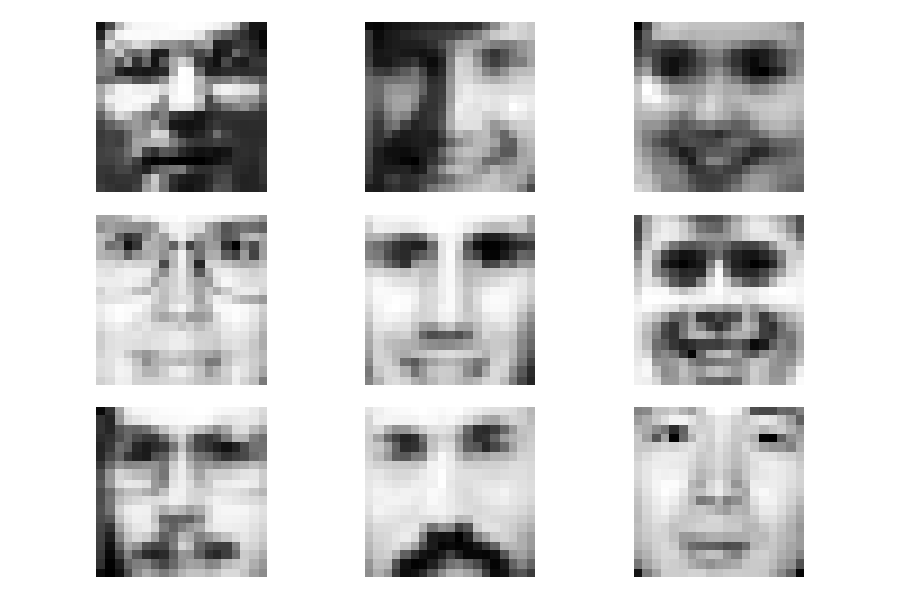
\includegraphics[width=0.32\textwidth]{Ex_03/Figures/imgs_k9.pdf}
\hfill
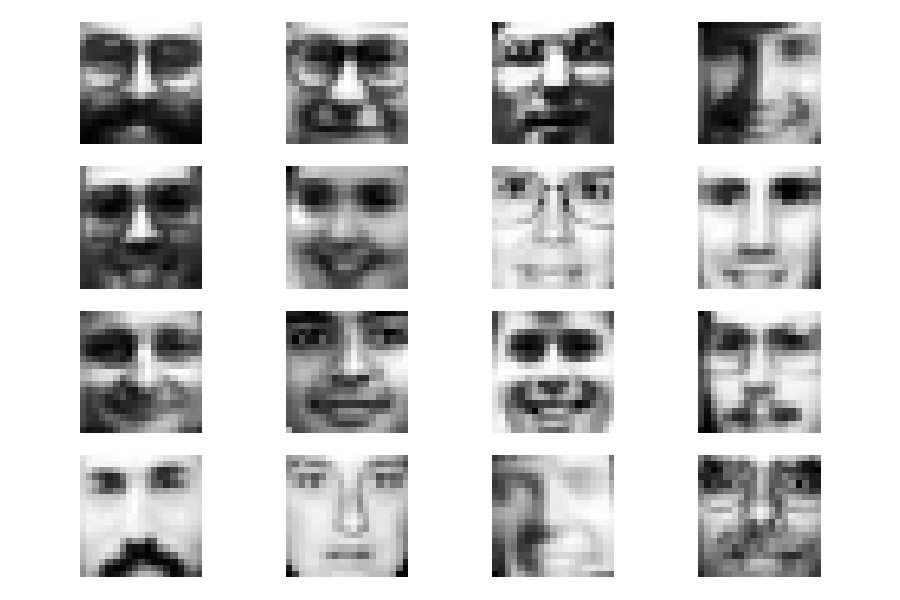
\includegraphics[width=0.32\textwidth]{Ex_03/Figures/imgs_k16.pdf}
\hfill
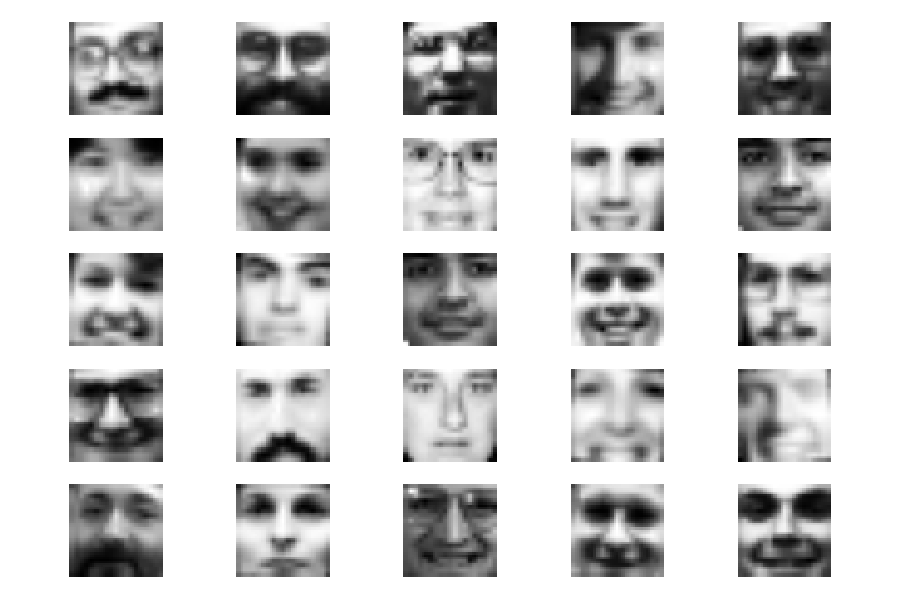
\includegraphics[width=0.32\textwidth]{Ex_03/Figures/imgs_k25.pdf}
\end{center}
%%%%%
%%%%%
%%%%%
%%%%%
%%%%%



